\chapter{Анализ основных причин джиттера в проводной и беспроводной сети} \label{chapt2}
Выделяют три типа джиттера \cite{clark}, которые могут быть вызваны различными причинами (рис. \ref{img:3typeJitter}):
\begin{enumerate}
  \item Выброс задержки возникает, когда один пакет в потоке оказывается задержанным на значительно больший интервал времени по отношению к другим. Это может произойти в тех случаях, когда осуществляется передача высокоприоритетного служебного трафика, когда возникают сетевые перегрузки, изменение маршрута и др. Эти случаи могут привести к проблеме неограниченного изменения оценки управляющей системы за один шаг.
  \item Постоянный джиттер - это передача пакетов с примерно постоянным изменением задержки;
  \item Скачок задержки, который может возникнуть из-за всплеска пакетной активности. Это явление, как правило, связано с перегрузками линии доступа или изменением маршрута. Скачок задержки может привести систему управления в неустойчивое состояние, что приводит к нежелательным последствиям.
\end{enumerate}

\begin{figure} [h] 
  \center
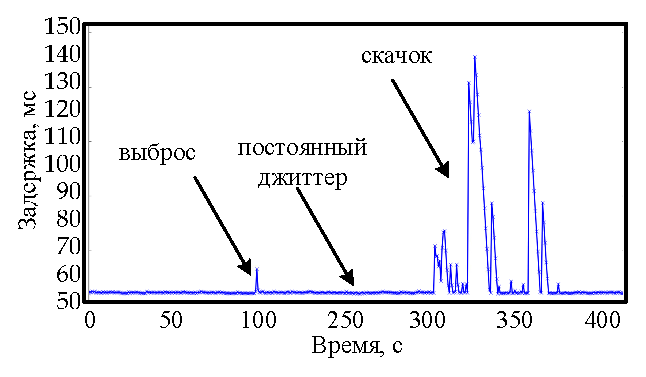
\includegraphics{3typeJitter.eps}
  %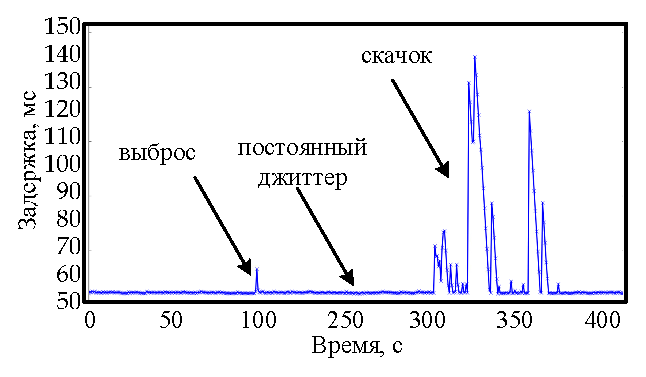
\includegraphics [scale=0.9] {3typeJitter.eps}
%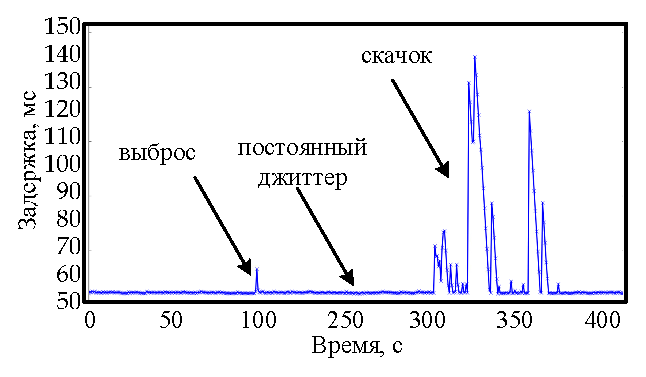
\includegraphics {3typeJitter}
  \caption{График задержек в реальной сети \cite{clark}} 
  \label{img:3typeJitter}  
\end{figure}
Различные типы джиттера, являются следствием различных сетевых ситуаций. В этом разделе будут рассмотрены основные причины возникновения различных типов джиттера в проводной и беспроводной сети.

\section{Анализ основных причин джиттера в проводной сети} \label{sect2_1}
\subsection{Пакетное планирование на стороне отправителя (тип 1)} \label{subsect2_1_1}
В некоторых системах, такие как программные телефоны, процессу VoIP приходится бороться за процессорное время с другими процессами и, следовательно, могут существовать некоторый джиттер времени передачи
\subsection{Перегрузка в локальной сети (тип 1)} \label{subsect2_1_2}
Хотя средняя загрузка локальной сети обычно не высокая, локальные перегрузки происходят в течение коротких периодов времени. Худший случай изменения задержки ограничен максимальным временем повторной попытки использовать сеть Ethernet, а в некоторых системах также ограничены межпакетной задержкой.
Если VoIP оконечная система не была в состоянии получить доступ к локальной сети, максимального времени отсрочки к запланированному моменту передачи следующего пакета, то пакет может быть отброшен. В случае 100 Мбит Ethernet максимальное время отсрочки находится в диапазоне миллисекунд и, следовательно, не должны быть основным источником джиттера. В случае 10 Мбит Ethernet максимальное время отсрочки значительно выше, чем расстояние между голосовыми пакетами и, следовательно, джиттер может быть ограничен расстоянием между пакетами, обычно на 10-30 мс.
Перегрузки в локальной сети обычно приводят выбросам задержки так, как один пакет может быть задержан, однако следующий пакет может сразу получить доступ к локальной сети (рис. \ref{img:localCongest}).

\begin{figure} [h]
  \center
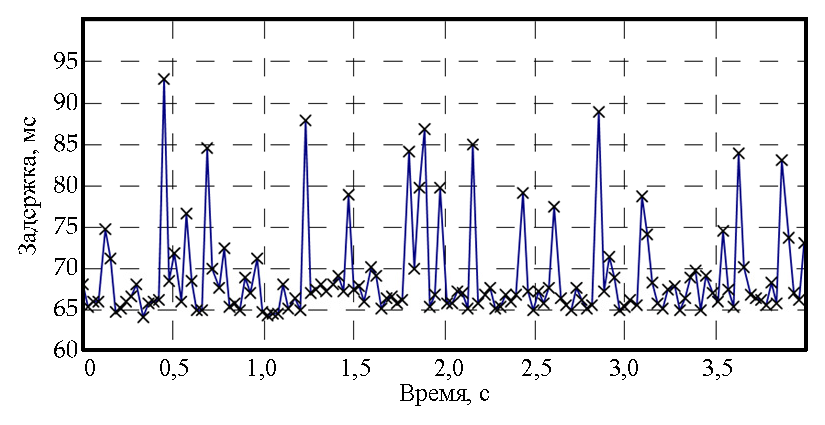
\includegraphics{localCongest.eps}
  \caption{Пример перегрузки в локальной сети \cite{clark}}
  \label{img:localCongest}
\end{figure}

\subsection{Перегрузки в канале доступа (тип 3) } \label{subsect2_1_3}
Доступ к каналу доступа, как правило, является одним из основных источников джиттера, поскольку он представляют собой одно из узких мест на пути пакета (рис. \ref{img:accessCongest}). Например, задержка сериализации IP-пакета в 1500 байт, посланного через T1 (1.544Mbit), будет около 8 миллисекунд, поэтому если в очереди перед речевой пакетом находятся пять пакетов данных, то вводится дополнительная задержка в 40 мс. Эта проблема может быть очень серьезной в случае ISDN, ADSL или в случае кабельных модемов, у которых пропускная способность исходящего канала дополнительно ограничена, например, если пропускная способность исходящего канала составляет 384кбит/в секунду, то каждый 1500 байтовый IP пакет в очереди введет дополнительную задержку в 30 мс.

\begin{figure} [h]
  \center
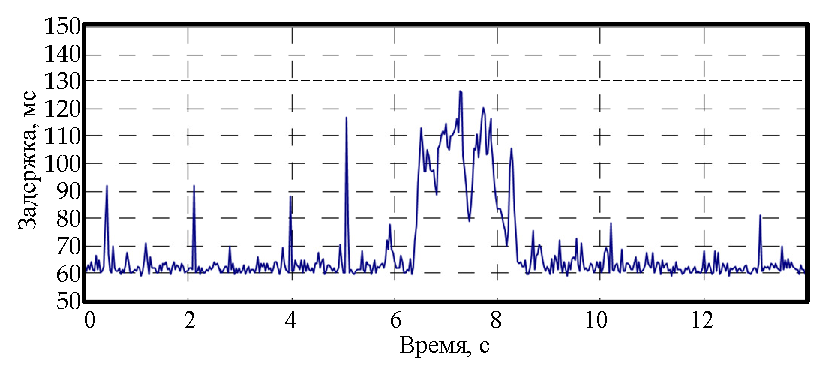
\includegraphics{accessCongest.eps}
  \caption{Пример перегрузки сети доступа \cite{clark}}
  \label{img:accessCongest}
\end{figure}

\subsection{Распределение нагрузки между несколькими линиями доступа или сервис провайдерами (тип 2) } \label{subsect2_1_4}
В целях предоставления предприятию VoIP доступа, предприятие может быть подключено через несколько сетей доступа к одному сервис провайдеру или направлять VoIP трафик через несколько независимых провайдеров. Это может привести к джиттеру если задержки на каждом канале доступа существенно различается.

\subsection{Распределение нагрузки (тип 2) } \label{subsect2_1_5}
Некоторые сервис провайдеры распределяют трафик через несколько внутренних маршрутов в пределах их сетей в целях повышения устойчивости и обеспечения более равномерной загрузки на сеть. Это вносит джиттер в результате разницы в задержке на каждом маршруте.

\subsection{Внутреннее разделение нагрузки в маршрутизаторах (тип 2) } \label{subsect2_1_6}
Для того чтобы поддерживать высокую скорость обработки некоторые маршрутизаторы используют многопроцессорные подход, при котором пакеты обрабатываются в нескольких параллельных очередях. Это может привести к небольшому уровню джиттера из-за различия в размере очереди.

\subsection{Высоко приоритетный служебный трафик (тип 1) } \label{subsect2_1_7}
Маршрутизаторы периодически генерируют трафик обновления с высоким приоритетом (рис. \ref{img:routeTraffic}) и выполняют обновления таблицы маршрутизации. Каждое такое событие может привести к задержке небольшого количества пакетов. Кроме того во время обновления таблицы маршрутизации могут существовать кратковременные петли, что может привести к чрезвычайно высокой задержке для отдельных пакетов (рис. \ref{img:routeChange}).

\begin{figure} [h]
  \center
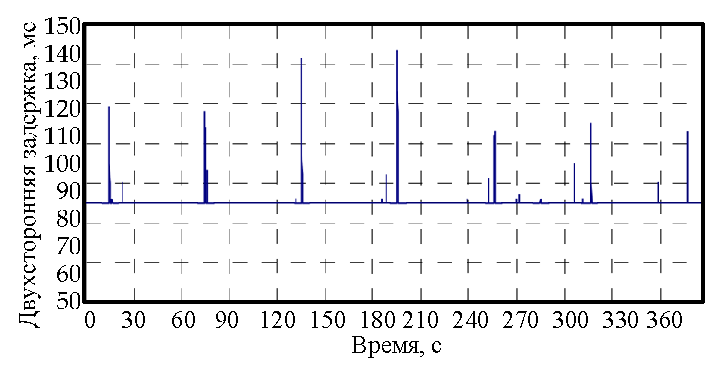
\includegraphics{routeTraffic.eps}
  \caption{Периодическое обновление таблицы маршрутизации без изменения маршрута \cite{clark}}
  \label{img:routeTraffic}
\end{figure}
\begin{figure} [h]
  \center
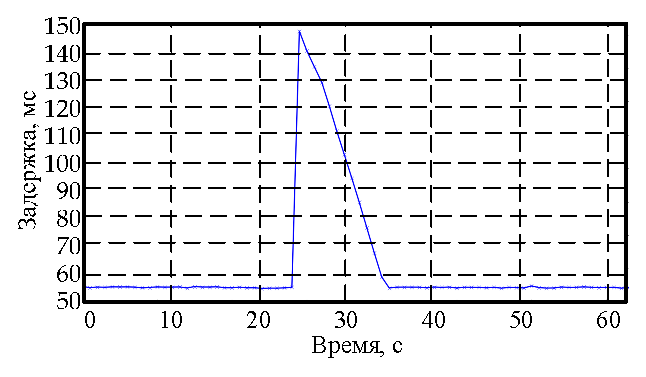
\includegraphics{routeChange.eps}
  \caption{Периодическое обновление таблицы маршрутизации при изменении маршрута \cite{clark}}
  \label{img:routeChange}
\end{figure}

\section{Анализ основных причин джиттера в беспроводной сети LTE} \label{sect2_2}
Беспроводная сеть налагает дополнительные факторы ухудшающие качество передачи. Далее рассмотрим влияние различных факторов на качество обслуживания, для услуг реального времени поверх сети LTE. Для моделирования и анализа ухудшающих факторов воспользуемся сетевым симмулятором NS3.

\subsection{Хэндовер}  \label{sect2_2_1}
Хэндовер (англ. Handover), является процессом передачи сессии абонента от одной базовой станции к другой. Может быть несколько причин для проведения передачи сессии:
\begin{itemize}
\item Когда абонент уходит с зоны покрытия одной ячейкой сети и входит в зону покрытия другой ячейкой. Хэндовер позволяет абонентам не быть привязанным к какой-либо географической точке и дает возможность передвигаться в пределах сети оператора без разрыва соединения.
\item Когда ёмкость сети в текущей ячейке израсходована при существовании соединения, которое находится в зоне, перекрытой другой ячейкой, передаётся к этой ячейке в порядке освобождения ёмкости первой ячейки для других ее пользователей, которые могут быть соединены только с первой ячейкой.
\item Когда канал используемый абонентом сильно зашумлён помехами, соединение передаётся другому каналу в той же ячейке или другому каналу в другой ячейке для устранения помех.
\item Когда абонент входит в зону микроячейки, соединение может быть передано для освобождения емкости большой сети.
\end{itemize}
Проведем моделирование влияния хэндовера на сквозную задержку в сети LTE в сетевом симмуляторе NS3. Детали стенда для моделирования описаны в Приложение \ref{AppendixA}. На рис. \ref{img:hand} избражено изменение сквозной сетевой задержки прибытия пакетов из-за 3-х переключений сессии абонента между базовыми станциями выполненными через некоторый промежуток времени. Также стоит заметить что при первой установке соединения задержка прибытия пакетов тоже была не стационарна.

\begin{figure} [h]
  \center
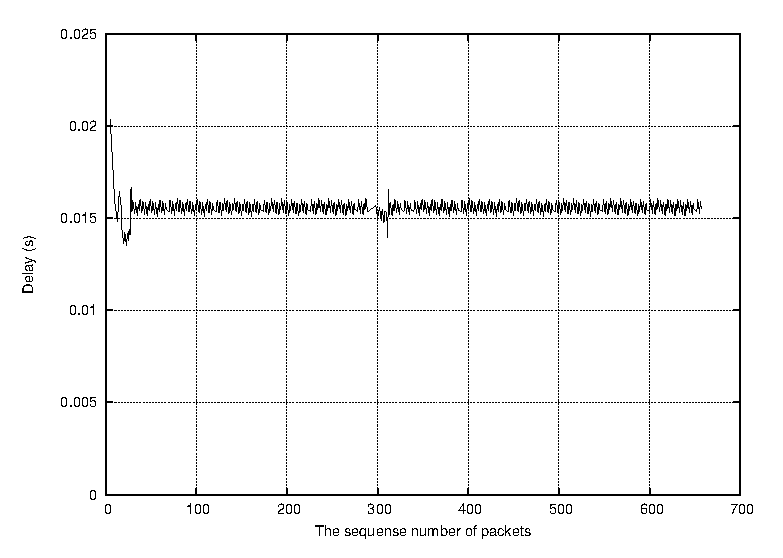
\includegraphics{hand.eps}
  \caption{Изменение задержки прибытия пакетов при хэндовере между базовыми станциями}
  \label{img:hand}
\end{figure}

\subsection{Расстояния между абонентом и базовой станцией}  \label{sect2_2_2}
Проведем моделирование влияния расстояния между абонентом и базовой станцией на скорость передачи в канале сети LTE в сетевом симмуляторе NS3. Детали стенда для моделирования описаны в Приложение \ref{AppendixB}. В моделировании воспользуемся моделью потерь сигнала при распространнени Фрииса, которая впервые была описана в \cite{Friis}. Данная модель описывается следующей простой формулой передачи для радиоканала состоящего из передающей и приемной антены в свободном пространстве:

\begin{equation}\label{eq:friisMod1}
\frac{P_{r}}{P_{t}}=\frac{A_{r}A_{t}}{d^{2}\lambda^{2}},
\end{equation}

\noindent где для случая с изотропной антеной, без тепловых потерь $A_{isotr.}=\frac{\lambda^{2}}{4\pi}$ получим следующие уравнение:

\begin{equation}\label{eq:friisMod2}
\frac{P_{r}}{P_{t}}=\frac{\lambda^{2}}{(4\pi d)^{2}},
\end{equation}

\noindent cовременным представлением этого уравнения является:

\begin{equation}\label{eq:friisNew}
P_{r}=\frac{P_{t}G_{t}G_{r}\lambda^{2}}{(4\pi d)^{2}L},
\end{equation}

\noindent где $P_{r}$ - мощность полученного сигнала (Вт), $P_{t}$ - мощность отправленного сигнала (Вт), $G_{t}$ - коэффициент передачи, $G_{r}$ - коэффициент приема, $\lambda$ - длина волны (м), $d$ - расстояние (м), $L$ - системные потери. Как ожидалось (рис. \ref{img:dist} (a)) с увеличением расстояния между абонентом и базовой станцией уменьшается отношение сигнал шум с внутриситемными помехами включительно (SINR). С   уменьшением SINR также уменьшается и MCS и TBS (рис. \ref{img:dist} (b,c))

Для расчета пропускной способности канала воспользуемся спектральной эффективностью $\eta_{i}$ из табл. \ref{MCS_spectr}  \cite{R1-081483}. Которая расчитывается по формуле:

\begin{equation}\label{eq:spectr1}
\eta_{i}=log_{2}(1+\frac{\gamma_{i}}{\Gamma}),
\end{equation}
\begin{equation}\label{eq:spectr2}
\Gamma=\frac{-ln(5\times BER}{1.5},
\end{equation}
\begin{equation}\label{eq:spectr3}
BER=0.00005.
\end{equation}

Расчитанная пропускная способность канала при ширине спектра канала  20МГц изображена на рис. \ref{img:dist} (d).

\clearpage

\begin{table} [htb]
  \centering
\parbox{15cm}{\caption{Соотношение спектральной эффективности ($\eta_{i}$) к индексу MCS ($I_{MCS}$)}\label{MCS_spectr}}
\begin{tabular}{|l|l|l|l|}
 \hline
 \hline
Спектральная эффективность($\eta_{i}$) & $Q_{m}$ & $R$        & MCS индекс ($I_{MCS}$) \\ \hline \hline 
\multicolumn{3}{|l|}{Reserved}  & 0 \\  \hline
    0.15234375     & 2  & 0.076172 & 1       \\ \hline
    0.193359375    & 2  & 0.09668  & 2       \\ \hline
    0.234375       & 2  & 0.117188 & 3       \\ \hline
    0.305664063    & 2  & 0.152832 & 4       \\ \hline
    0.376953125    & 2  & 0.188477 & 5       \\ \hline
    0.489257813    & 2  & 0.244629 & 6       \\ \hline
    0.6015625      & 2  & 0.300781 & 7       \\ \hline
    0.739257813    & 2  & 0.369629 & 8       \\ \hline
    0.876953125    & 2  & 0.438477 & 9       \\ \hline
    1.026367188    & 2  & 0.513184 & 10      \\ \hline
    1.17578125     & 2  & 0.587891 & 11      \\ \hline
    1.326171875    & 4  & 0.331543 & 12      \\ \hline
    1.4765625      & 4  & 0.369141 & 13      \\ \hline
    1.6953125      & 4  & 0.423828 & 14      \\ \hline
    1.9140625      & 4  & 0.478516 & 15      \\ \hline
    2.16015625     & 4  & 0.540039 & 16      \\ \hline
    2.40625        & 4  & 0.601563 & 17      \\ \hline
    2.568359375    & 4  & 0.64209  & 18      \\ \hline
    2.73046875     & 6  & 0.455078 & 19      \\ \hline
    3.026367188    & 6  & 0.504395 & 20      \\ \hline
    3.322265625    & 6  & 0.553711 & 21      \\ \hline
    3.612304688    & 6  & 0.602051 & 22      \\ \hline
    3.90234375     & 6  & 0.650391 & 23      \\ \hline
    4.212890625    & 6  & 0.702148 & 24      \\ \hline
    4.5234375      & 6  & 0.753906 & 25      \\ \hline
    4.819335938    & 6  & 0.803223 & 26      \\ \hline
    5.115234375    & 6  & 0.852539 & 27      \\ \hline
    5.334960938    & 6  & 0.88916  & 28      \\ \hline
    5.5546875      & 6  & 0.925781 & 29      \\ \hline
    2.4            & 2  & 1.2      & 30      \\ \hline
\multicolumn{3}{|l|}{Reserved}  & 31 \\  \hline
    \end{tabular}
\end{table}

\clearpage

\begin{figure} [!h]
\begin{minipage}[h]{0.47\linewidth}
\center
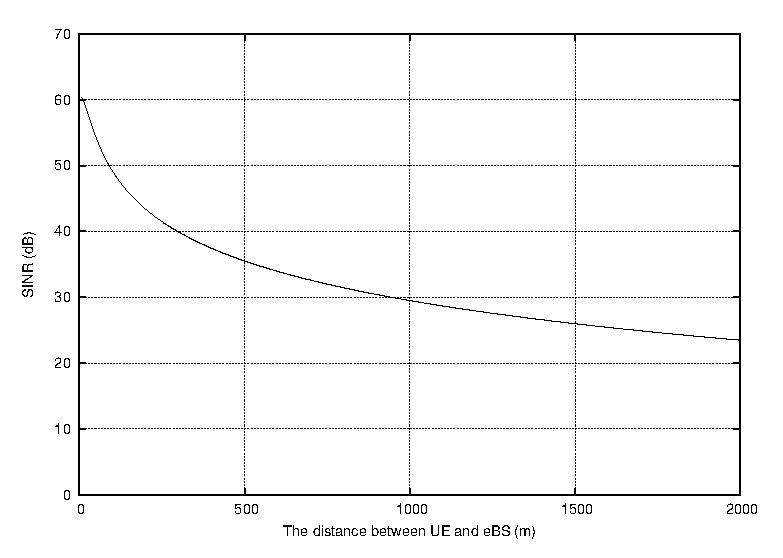
\includegraphics[width=1\linewidth]{Sinr_dist.eps} a) \\
\end{minipage}
\hfill
\begin{minipage}[h]{0.47\linewidth}
\center
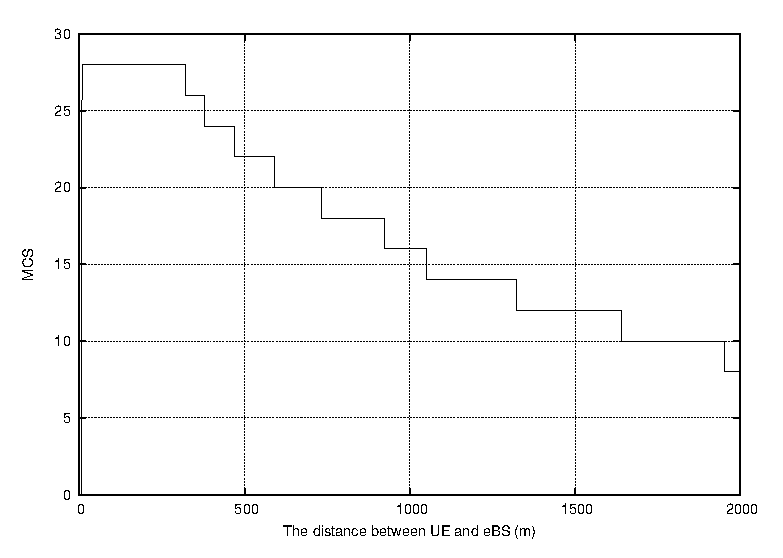
\includegraphics[width=1\linewidth]{mcs_dist.eps} b) \\
\end{minipage}
\vfill
\begin{minipage}[h]{0.47\linewidth}
\center
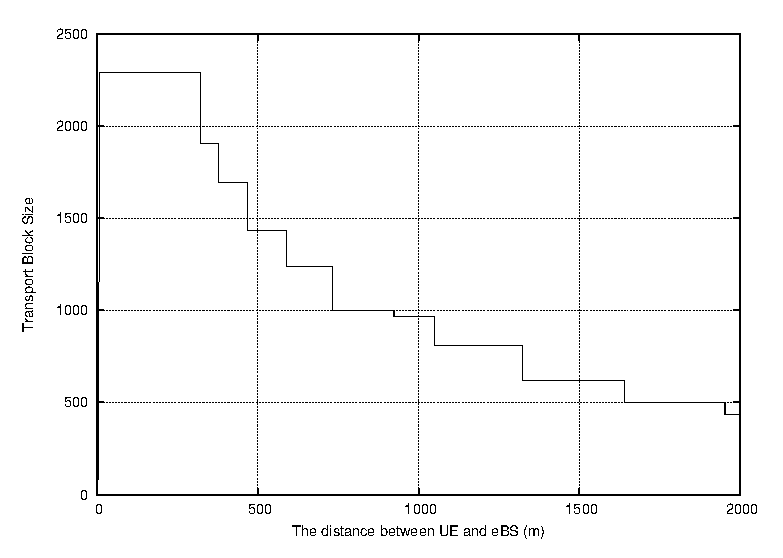
\includegraphics[width=1\linewidth]{tb_dist.eps} c) \\
\end{minipage}
\hfill
\begin{minipage}[h]{0.47\linewidth}
\center
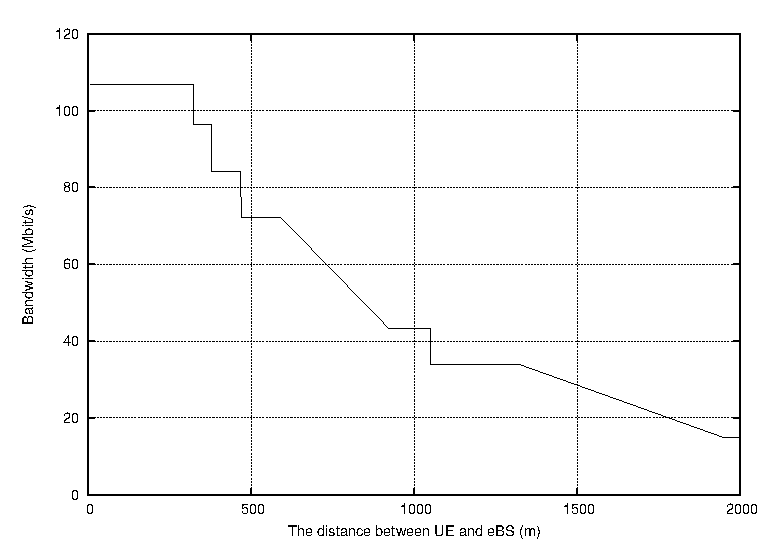
\includegraphics[width=1\linewidth]{speed_dist.eps} d) \\
\end{minipage}
\caption{Зависимость a) SINR b) MCS c) размера TBS d) скорости передачи нисходяшего канала передачи от растояния между абонентом и базовой станцией}
\label{img:dist}
\end{figure}

\subsection{Внутрисистемные помехи}  \label{sect2_2_3}
Рассмотрим влияние всплесков внутрисистемных помех на характеристики канала передаци в сети LTE. Всплеск внутрисистемных помех может быть вызван другой базовой станцией, которая работает в том же диапазоне, хотя воздействие не зависит от источника помех.
Анализ описывает, как всплески помех влияет на характеристики канала в том числе на джиттер и  потери пакетов.

Для борьбы с помехами электромагнитной несовместимости используется помехоустойчивое кодирование и перемежение. Тем не менее, блоковые ошибки возникают, когда условия канала достаточно плохи. Это приводит к потери пакетов для IP услуг, таких как FTP и VoIP. LTE использует повторные передачи чтобы поддерживать определенный уровень потери пакетов, что может быть не достаточно эффектиыным, чтобы предоставить хорошее качество для соответствующей услуги. Результат применения повторной передачи является джиттер задержки.
LTE передачи часто запланированы таким образом, чтобы быть синхронизированными с качеством канала, таким образом, что пакеты передавались к и от пользователей, имеющих наилучшие канальные условия, а пользователи, которые испытывают провалы качества канала, будут ожидать пока условия канала не будут улучшены. Это означает, что пакеты в очереди передачи будут испытывать различные задержки из-за планирования.
LTE также ограничивает количество повторных передач, чтобы избежать использования слишком большого количества ресурсов передачи для пользователей, которые испытывают деградацию характеристик канала. Это означает, что потери пакетов могут происходить в дополнение джиттеру задержки. Для услуг в реального времени, характерно чтобы пакеты могли быть повторно переданы со сквозной задержкой передачи до 50-100 мс.
Концептуальный пример задержки пакетов, которые могут произойти в присутствии внутрисистемных помех, показан на рис \ref{img:example_inter}.


\pgfplotsset{width=15cm, height=10cm, compat=1.3}
\begin{figure} [h]
  \center
\begin{tikzpicture}
\begin{axis}[
xlabel=Номер пакета,
ylabel=Задержка пакета (мс)]
\addplot [only marks, color=blue ,mark=x] coordinates {
( 1, 150 )
( 2, 150 )
( 3, 150 )
( 4, 150 )
( 5, 150 )
( 6, 150 )
( 7, 150 )
( 8, 150 )
( 9, 150 )
( 13, 250 )
( 14, 230 )
( 15, 210 )
( 16, 190 )
( 17, 170 )
( 19, 150 )
( 20, 150 )
( 21, 150 )
( 22, 150 )
( 21, 150 )
( 22, 150 )
( 23, 150 )
( 24, 150 )
( 25, 150 )
( 26, 150 )
( 27, 150 )
( 28, 150 )
( 29, 150 )
( 30, 150 )


};
\addplot [only marks, color=red] coordinates {
( 10, 0 )
( 11, 0 )
( 12, 0 )};
\legend{Задержка пакета, Потеря пакета}
\end{axis}
\end{tikzpicture}
\caption{Концептуальный пример времени прибытия IP пакетов (синие маркеры), потерь пакетов (красные маркеры) и джиттера задержки в присутствии сильного всплеска внутрисистемных помех.}
  \label{img:example_inter}
\end{figure}


Следующие поведение можно ожидать, если позволено планирование передачи пакетов и повторное время передачи короче, чем период помехи:
Перед помехой, пакеты передаются без или почти без джиттера. В этом концептуальном  примере предполагается что постоянный джиттер отсутствует, чтобы выделить вклад в характеристики канала, вызванный внутрисистемной помехой радара.
На начальном этапе воздействия помехи вполне вероятно, что пакеты будут потеряны. Это происходит из-за ограничений в планировании передачи пакетов и ограничений времени повторной передачи, как описано выше.
Пакеты сгенерированные в конце периода воздействия помехи будут поставлены в очередь. Передатчик может попытаться отправить эти пакеты, но вполне вероятно, что передача будет успешной только после окончания периода помехи. Это может привести к большим задержкам этих пакетов. Вероятным следствием длительных задержек пакетов является то, что буферу компенсации джиттера возможно придется отказаться от пакетов, которые пришли слишком поздно, чтобы быть использованными для декодирования.
После периода воздействия помехи задержки пакетов медленно снижаются. Это потому, что пакеты, которые сгенерированные непосредственно после помехи еще ожидают в очереди передачи.
Передача вернется к нормальному состоянию, когда передатчик очистит очередь передачи.
Такое поведение, то есть джиттер и потери пакетов называется "скачок задержки" и является довольно частым явлением в пакетно коммутируемой сотовой сети, которая использует повторные передач. Величина потерь пакетов и размер скачка задержки зависит как от помехи так и от того как система настроена.

Проведем экспримент в NS3 для демонстрации влияния внутрисистемных помех в LTE. Схема эксперимента изображена на рис. \ref{img:inter_schem}. С уменьшением расстояния до источника помехи, мощьность помехи увеличивается и характеристи канала деградируют (рис. \ref{img:inter})
\begin{figure} [h]
  \center
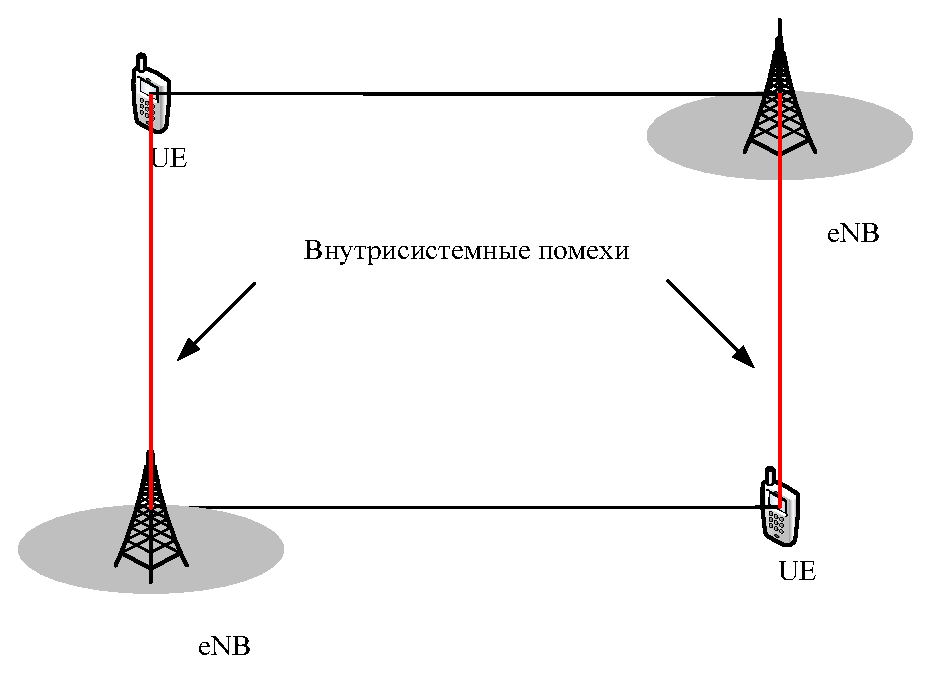
\includegraphics[width=0.8\linewidth]{inter_schem.eps}
  \caption{Схема моделирования влияния внутрисистемных помех в NS3}
  \label{img:inter_schem}
\end{figure}
\begin{figure} [h]
\begin{minipage}[h]{0.47\linewidth}
\center
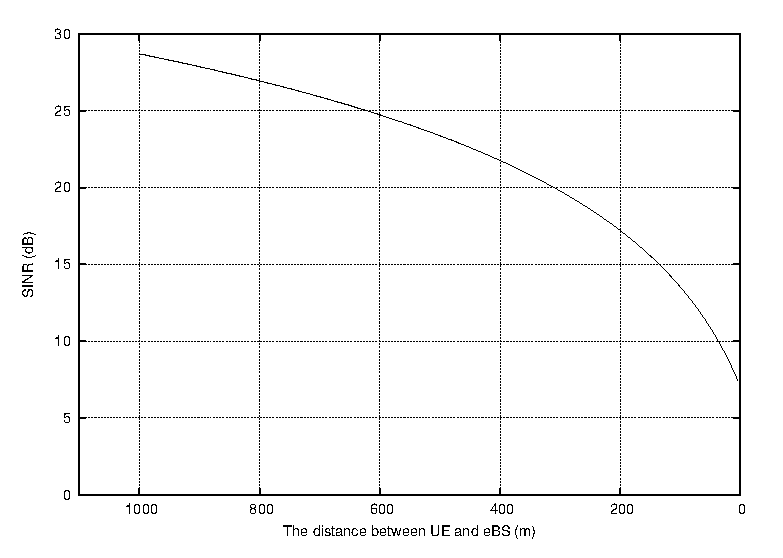
\includegraphics[width=1\linewidth]{Sinr_inter.eps} a) \\
\end{minipage}
\hfill
\begin{minipage}[h]{0.47\linewidth}
\center
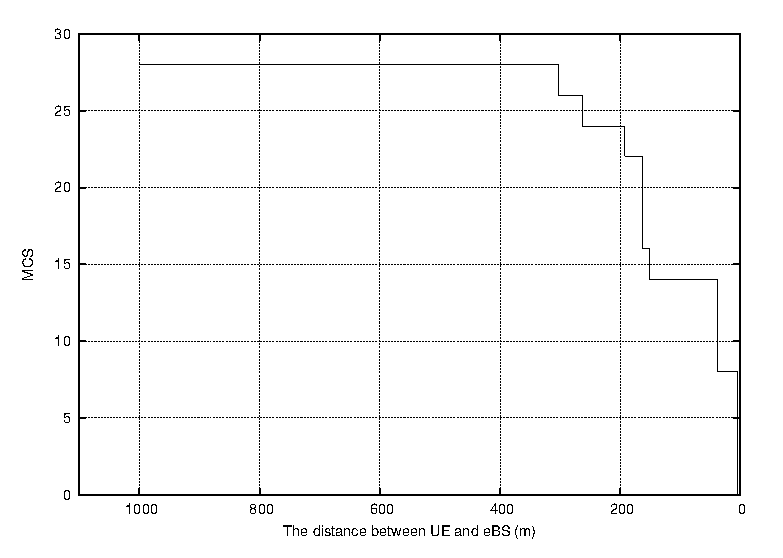
\includegraphics[width=1\linewidth]{mcs_inter.eps} b) \\
\end{minipage}
\vfill
\begin{minipage}[h]{0.47\linewidth}
\center
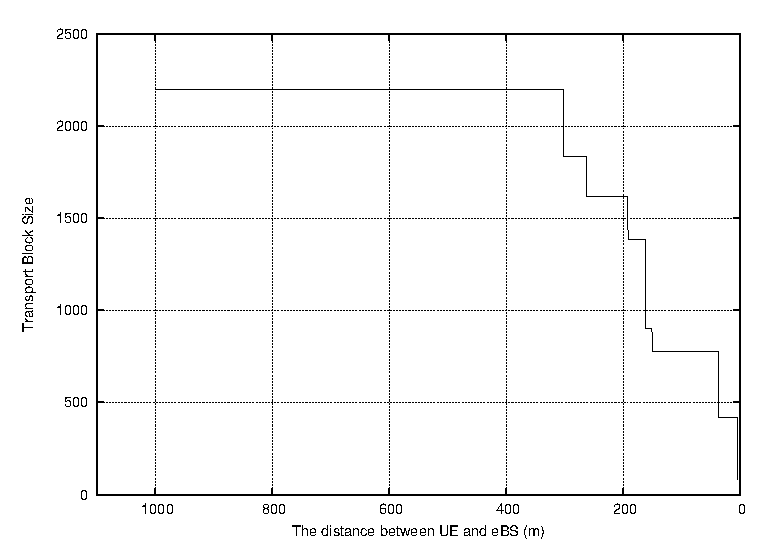
\includegraphics[width=1\linewidth]{tb_inter.eps} c) \\
\end{minipage}
\hfill
\begin{minipage}[h]{0.47\linewidth}
\center
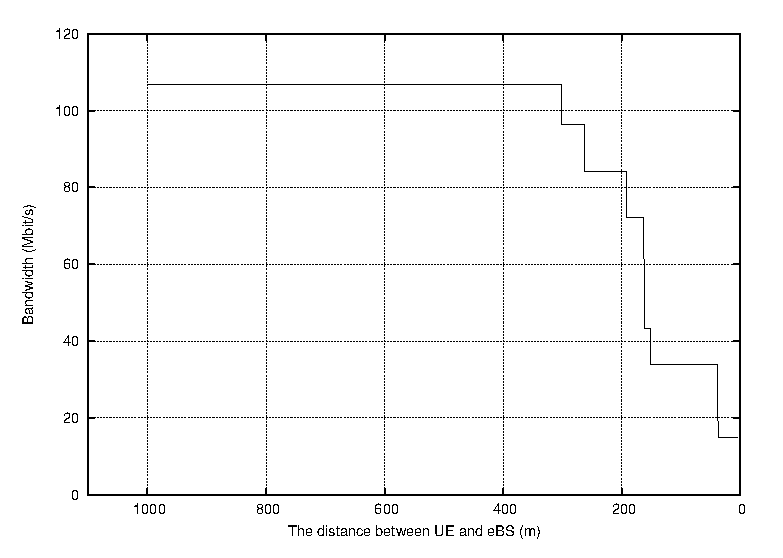
\includegraphics[width=1\linewidth]{speed_inter.eps} d) \\
\end{minipage}
\caption{Зависимость a) SINR b) MCS c) размера TB d) скорости передачи нисходяшего канала передачи от растояния между абонентом и помеховой базовой станцией}
\label{img:inter}
\end{figure}

%\clearpage


\subsection{Замирания в канале}  \label{sect2_2_4}
Работа LTE-приемника зависит от разных факторов: конкретного частотного диапазона, многолучевых задержек, доплеровских сдвигов частоты, реализации технологии множественного приема/передачи (MIMO) и т.д.

В реальной среде такие объекты, как горы, здания и машины, отражают, преломляют или не пропускают передаваемые радиосигналы. Эти объекты могут располагаться на различном расстоянии от передатчика – одни ближе, другие дальше. Вследствие этого множество копий сигнала достигают антенны приемника за разное время. У таких запаздывающих копий разные фазовые соотношения, которые при приеме дают как положительный, так и отрицательный эффект. Незначительные отклонения в фазовых соотношениях вызывают пешеходы и машины. Если абонентский терминал перемещается, то изменение фазы увеличивается с ростом его скорости.

Эксперименты показывают колебания уровня принимаемого сигнала выше или ниже его номинала; иногда он снижается до очень низких, почти нулевых значений.

При движении передатчика или приемника проявляется другой эффект – доплеровский сдвиг частоты. Так как запаздывающие копии сигнала поступают на приемник с разных относительно вектора движения направлений, частоты некоторых из них сдвигаются – одни выше, другие ниже реальной частоты сигнала. Этот эффект вызывает особые сложности в OFDM-системах, поскольку для устранения интерференции внутренних поднесущих нельзя использовать простой сдвиг частоты.

По мере увеличения количества путей распространения сигнала растет и число наложений его копий с разными синхронизацией, амплитудой, частотой и фазой. В результате сигнал становится стохастическим (недетерминированным) с рэлеевским распределением. Как известно, рэлеевское распределение точно отражает колебания амплитуды и изменения частоты (называемые еще доплеровским расширением), характерные для городской застройки.

Условия распространения характеризуются тремя факторами: профилем многолучевой задержки, доплеровским расширением и, в случае применения нескольких антенн, – набором коррелирующих матриц, задающих соотношения для передающей и приемной антенн.

Профиль задержки определяет количество путей распространения, саму задержку и ослабление сигнала. Кроме того, по этому профилю можно вычислить среднеквадратичное отклонение (разброс) задержки. Для технологии LTE выбраны три профиля: для пешехода (табл. \ref{EPA}), мобильного пользователя в автомобиле (табл. \ref{EVA}) и для типовой городской застройки (табл. \ref{ETU}). Сумартная информация по профилям задержек для технологии LTE находится в табл. \ref{ProfileDelay}.



\begin{table} [htb]
  \centering
\parbox{15cm}{\caption{Расширенная А модель пешехода (ЕРА) \cite{TS36104}}\label{EPA}}
\begin{tabular}{|l|l|}
    \hline
    \hline
    Задержка за счет отклонения от трассы в нс &  Соответсвующая мощность в дБ \\ \hline \hline
    0                                     & 0.0                           \\ \hline
    30                                    & -1.0                          \\ \hline
    70                                    & -2.0                          \\ \hline
    90                                    & -3.0                          \\ \hline
    110                                   & -8.0                          \\ \hline
    190                                   & -17.2                         \\ \hline
    410                                   & -20.8                         \\ \hline
    \end{tabular}

\end{table}

\begin{table} [htb]
  \centering
\parbox{15cm}{\caption{Расширенная А-модель при движении при движении в автомобиле (EVA) \cite{TS36104}}\label{EVA}}
\begin{tabular}{|l|l|}
    \hline
    \hline
    Задержка за счет отклонения от трассы в нс &  Соответсвующая мощность в дБ \\ \hline \hline
    0                                          & 0.0                           \\ \hline
    30                                         & -1.5                          \\ \hline
    150                                        & -1.4                          \\ \hline
    310                                        & -3.6                          \\ \hline
    370                                        & -0.6                          \\ \hline
    710                                        & -9.1                          \\ \hline
    1090                                       & -7.0                          \\ \hline
    1730                                       & -12.0                         \\ \hline
    2510                                       & -16.9                         \\ \hline
    \end{tabular}
\end{table}


\begin{table} [htb]
  \centering
\parbox{15cm}{\caption{Расширенная модель для типовой городской застройки (ETU) \cite{TS36104}}\label{ETU}}
\begin{tabular}{|l|l|}
    \hline
    \hline
    Задержка за счет отклонения от трассы в нс &  Соответсвующая мощность в дБ \\ \hline \hline
    0    & -1.0 \\ \hline
    50   & -1.0 \\ \hline
    120  & -1.0 \\ \hline
    200  & 0.0  \\ \hline
    230  & 0.0  \\ \hline
    500  & 0.0  \\ \hline
    1600 & -3.0 \\ \hline
    2300 & -5.0 \\ \hline
    5000 & -7.0 \\ \hline
    \end{tabular}
\end{table}



\begin{table} [htb]
  \centering
\parbox{15cm}{\caption{Профили задержеки для технлогии LTE \cite{iks}}\label{ProfileDelay}}
    \begin{tabular}{|p{5cm}|p{3cm}|p{3cm}|p{4cm}|}
    \hline \hline
    Модель                                                            &  Количество путей в канале &  Разброс задержки в нс &  Максимальная задержка по траектории в нс \\ \hline \hline
    Расширенная А-модель пешехода (ЕРА)                               & 7                          & 45                     & 410                                       \\ \hline
    Расширенная А-модель при движении при движении в автомобиле (EVA) & 9                          & 367                    & 2510                                      \\ \hline
    Расширенная модель для типовой городской застройки (ETU)          & 9                          & 991                    & 5000                                      \\ \hline
    \end{tabular}
\end{table}



Еще один параметр – максимальная величина доплеровского сдвига частоты. Максимальный доплеровский сдвиг происходит для волны, идущей в противоположном направлении направлению движения антенны. Он имеет частотный сдвиг:

\begin{equation}\label{eq:maxDeltaF}
f_{D}=\frac{\mathcal{V}}{c}-f_{c},
\end{equation}
\noindent где $f_{c}$ является несущей частотой, $\mathcal{V}$ - скорость движения антены и $c$ - скорость света. Все пути в канале имеют классический доплеровский спек
тр плотности мощности:

\begin{equation}\label{eq:maxDeltaF}
S(f)=\frac{1}{\pi f_D \sqrt{1-(\frac{f}{f_D})^2}},
\end{equation}
\noindent где $f\epsilon [-f_D;f_D]$. Для LTE-сетей обычно применяются три значения: 5 Гц, 70 Гц и 300 Гц – для низко, средне и высокоскоростных объектов. При работе в диапазоне 2 ГГц эти частоты соответствуют следующим скоростям движения пользователя терминала: 2,7 км/ч, 38,4 км/ч и 162 км/ч. Требования к работе приемника формируются с учетом комбинации этих доплеровских сдвигов частоты с профилями задержки. И хотя существуют три профиля и три доплеровских сдвига частоты, из возможных сочетаний используются лишь пять (табл. \ref{model_chanel}). Профиль пешехода как низкоскоростного объекта определен только для частоты 5 Гц; профиль пользователя в автомобиле – для 5 и 70 Гц, а типовой профиль для города не включает частоту 5 Гц.


\begin{table} [htb]
  \centering
\parbox{15cm}{\caption{Параметры модели канала \cite{iks}}\label{model_chanel}}
\begin{tabular}{|l|c|}
    \hline
    \hline
    Модель     & Максимальный доплеровский сдвиг частоты, Гц \\ \hline \hline
    ЕРА 5 Гц   & 5                                       \\ \hline
    EVA 5 Гц   & 5                                       \\ \hline
    EVA 70 Гц  & 70                                      \\ \hline
    ETU 70 Гц  & 70                                      \\ \hline
    ETU 300 Гц & 300                                     \\ \hline
    \end{tabular}
\end{table}



\begin{figure} [H]
\begin{minipage}[h]{0.47\linewidth}
\center
\includegraphics[width=1\linewidth]{EPA_3kmph/Sinr_fading.eps} a) \\
\end{minipage}
\hfill
\begin{minipage}[h]{0.47\linewidth}
\center
\includegraphics[width=1\linewidth]{EPA_3kmph/mcs_fading.eps} b) \\
\end{minipage}
\vfill
\begin{minipage}[h]{0.47\linewidth}
\center
\includegraphics[width=1\linewidth]{EPA_3kmph/tb_fading.eps} c) \\
\end{minipage}
\hfill
\begin{minipage}[h]{0.47\linewidth}
\center
\includegraphics[width=1\linewidth]{EPA_3kmph/speed_fading.eps} d) \\
\end{minipage}
\caption{Влияние замираний на a) SINR b) MCS c) размер TB d) скорость передачи нисходяшего канала передачи при пешеходном сценарии (0-3 км/ч)}
\label{img:EPA_3kmph}
\end{figure}

\begin{figure} [H]
\begin{minipage}[h]{0.47\linewidth}
\center
\includegraphics[width=1\linewidth]{EVA_60kmph/Sinr_fading.eps} a) \\
\end{minipage}
\hfill
\begin{minipage}[h]{0.47\linewidth}
\center
\includegraphics[width=1\linewidth]{EVA_60kmph/mcs_fading.eps} b) \\
\end{minipage}
\vfill
\begin{minipage}[h]{0.47\linewidth}
\center
\includegraphics[width=1\linewidth]{EVA_60kmph/tb_fading.eps} c) \\
\end{minipage}
\hfill
\begin{minipage}[h]{0.47\linewidth}
\center
\includegraphics[width=1\linewidth]{EVA_60kmph/speed_fading.eps} d) \\
\end{minipage}
\caption{Влияние замираний на a) SINR b) MCS c) размер TB d) скорость передачи нисходяшего канала передачи при автомобильном сценарии (30-60 км/ч)}
\label{img:EVA_60kmph}
\end{figure}




\clearpage




